% Options for packages loaded elsewhere
% Options for packages loaded elsewhere
\PassOptionsToPackage{unicode}{hyperref}
\PassOptionsToPackage{hyphens}{url}
\PassOptionsToPackage{dvipsnames,svgnames,x11names}{xcolor}
%
\documentclass[
  letterpaper,
  DIV=11,
  numbers=noendperiod]{scrartcl}
\usepackage{xcolor}
\usepackage{amsmath,amssymb}
\setcounter{secnumdepth}{-\maxdimen} % remove section numbering
\usepackage{iftex}
\ifPDFTeX
  \usepackage[T1]{fontenc}
  \usepackage[utf8]{inputenc}
  \usepackage{textcomp} % provide euro and other symbols
\else % if luatex or xetex
  \usepackage{unicode-math} % this also loads fontspec
  \defaultfontfeatures{Scale=MatchLowercase}
  \defaultfontfeatures[\rmfamily]{Ligatures=TeX,Scale=1}
\fi
\usepackage{lmodern}
\ifPDFTeX\else
  % xetex/luatex font selection
\fi
% Use upquote if available, for straight quotes in verbatim environments
\IfFileExists{upquote.sty}{\usepackage{upquote}}{}
\IfFileExists{microtype.sty}{% use microtype if available
  \usepackage[]{microtype}
  \UseMicrotypeSet[protrusion]{basicmath} % disable protrusion for tt fonts
}{}
\makeatletter
\@ifundefined{KOMAClassName}{% if non-KOMA class
  \IfFileExists{parskip.sty}{%
    \usepackage{parskip}
  }{% else
    \setlength{\parindent}{0pt}
    \setlength{\parskip}{6pt plus 2pt minus 1pt}}
}{% if KOMA class
  \KOMAoptions{parskip=half}}
\makeatother
% Make \paragraph and \subparagraph free-standing
\makeatletter
\ifx\paragraph\undefined\else
  \let\oldparagraph\paragraph
  \renewcommand{\paragraph}{
    \@ifstar
      \xxxParagraphStar
      \xxxParagraphNoStar
  }
  \newcommand{\xxxParagraphStar}[1]{\oldparagraph*{#1}\mbox{}}
  \newcommand{\xxxParagraphNoStar}[1]{\oldparagraph{#1}\mbox{}}
\fi
\ifx\subparagraph\undefined\else
  \let\oldsubparagraph\subparagraph
  \renewcommand{\subparagraph}{
    \@ifstar
      \xxxSubParagraphStar
      \xxxSubParagraphNoStar
  }
  \newcommand{\xxxSubParagraphStar}[1]{\oldsubparagraph*{#1}\mbox{}}
  \newcommand{\xxxSubParagraphNoStar}[1]{\oldsubparagraph{#1}\mbox{}}
\fi
\makeatother

\usepackage{color}
\usepackage{fancyvrb}
\newcommand{\VerbBar}{|}
\newcommand{\VERB}{\Verb[commandchars=\\\{\}]}
\DefineVerbatimEnvironment{Highlighting}{Verbatim}{commandchars=\\\{\}}
% Add ',fontsize=\small' for more characters per line
\usepackage{framed}
\definecolor{shadecolor}{RGB}{241,243,245}
\newenvironment{Shaded}{\begin{snugshade}}{\end{snugshade}}
\newcommand{\AlertTok}[1]{\textcolor[rgb]{0.68,0.00,0.00}{#1}}
\newcommand{\AnnotationTok}[1]{\textcolor[rgb]{0.37,0.37,0.37}{#1}}
\newcommand{\AttributeTok}[1]{\textcolor[rgb]{0.40,0.45,0.13}{#1}}
\newcommand{\BaseNTok}[1]{\textcolor[rgb]{0.68,0.00,0.00}{#1}}
\newcommand{\BuiltInTok}[1]{\textcolor[rgb]{0.00,0.23,0.31}{#1}}
\newcommand{\CharTok}[1]{\textcolor[rgb]{0.13,0.47,0.30}{#1}}
\newcommand{\CommentTok}[1]{\textcolor[rgb]{0.37,0.37,0.37}{#1}}
\newcommand{\CommentVarTok}[1]{\textcolor[rgb]{0.37,0.37,0.37}{\textit{#1}}}
\newcommand{\ConstantTok}[1]{\textcolor[rgb]{0.56,0.35,0.01}{#1}}
\newcommand{\ControlFlowTok}[1]{\textcolor[rgb]{0.00,0.23,0.31}{\textbf{#1}}}
\newcommand{\DataTypeTok}[1]{\textcolor[rgb]{0.68,0.00,0.00}{#1}}
\newcommand{\DecValTok}[1]{\textcolor[rgb]{0.68,0.00,0.00}{#1}}
\newcommand{\DocumentationTok}[1]{\textcolor[rgb]{0.37,0.37,0.37}{\textit{#1}}}
\newcommand{\ErrorTok}[1]{\textcolor[rgb]{0.68,0.00,0.00}{#1}}
\newcommand{\ExtensionTok}[1]{\textcolor[rgb]{0.00,0.23,0.31}{#1}}
\newcommand{\FloatTok}[1]{\textcolor[rgb]{0.68,0.00,0.00}{#1}}
\newcommand{\FunctionTok}[1]{\textcolor[rgb]{0.28,0.35,0.67}{#1}}
\newcommand{\ImportTok}[1]{\textcolor[rgb]{0.00,0.46,0.62}{#1}}
\newcommand{\InformationTok}[1]{\textcolor[rgb]{0.37,0.37,0.37}{#1}}
\newcommand{\KeywordTok}[1]{\textcolor[rgb]{0.00,0.23,0.31}{\textbf{#1}}}
\newcommand{\NormalTok}[1]{\textcolor[rgb]{0.00,0.23,0.31}{#1}}
\newcommand{\OperatorTok}[1]{\textcolor[rgb]{0.37,0.37,0.37}{#1}}
\newcommand{\OtherTok}[1]{\textcolor[rgb]{0.00,0.23,0.31}{#1}}
\newcommand{\PreprocessorTok}[1]{\textcolor[rgb]{0.68,0.00,0.00}{#1}}
\newcommand{\RegionMarkerTok}[1]{\textcolor[rgb]{0.00,0.23,0.31}{#1}}
\newcommand{\SpecialCharTok}[1]{\textcolor[rgb]{0.37,0.37,0.37}{#1}}
\newcommand{\SpecialStringTok}[1]{\textcolor[rgb]{0.13,0.47,0.30}{#1}}
\newcommand{\StringTok}[1]{\textcolor[rgb]{0.13,0.47,0.30}{#1}}
\newcommand{\VariableTok}[1]{\textcolor[rgb]{0.07,0.07,0.07}{#1}}
\newcommand{\VerbatimStringTok}[1]{\textcolor[rgb]{0.13,0.47,0.30}{#1}}
\newcommand{\WarningTok}[1]{\textcolor[rgb]{0.37,0.37,0.37}{\textit{#1}}}

\usepackage{longtable,booktabs,array}
\newcounter{none} % for unnumbered tables
\usepackage{calc} % for calculating minipage widths
% Correct order of tables after \paragraph or \subparagraph
\usepackage{etoolbox}
\makeatletter
\patchcmd\longtable{\par}{\if@noskipsec\mbox{}\fi\par}{}{}
\makeatother
% Allow footnotes in longtable head/foot
\IfFileExists{footnotehyper.sty}{\usepackage{footnotehyper}}{\usepackage{footnote}}
\makesavenoteenv{longtable}
\usepackage{graphicx}
\makeatletter
\newsavebox\pandoc@box
\newcommand*\pandocbounded[1]{% scales image to fit in text height/width
  \sbox\pandoc@box{#1}%
  \Gscale@div\@tempa{\textheight}{\dimexpr\ht\pandoc@box+\dp\pandoc@box\relax}%
  \Gscale@div\@tempb{\linewidth}{\wd\pandoc@box}%
  \ifdim\@tempb\p@<\@tempa\p@\let\@tempa\@tempb\fi% select the smaller of both
  \ifdim\@tempa\p@<\p@\scalebox{\@tempa}{\usebox\pandoc@box}%
  \else\usebox{\pandoc@box}%
  \fi%
}
% Set default figure placement to htbp
\def\fps@figure{htbp}
\makeatother





\setlength{\emergencystretch}{3em} % prevent overfull lines

\providecommand{\tightlist}{%
  \setlength{\itemsep}{0pt}\setlength{\parskip}{0pt}}



 


\KOMAoption{captions}{tableheading}
\makeatletter
\@ifpackageloaded{caption}{}{\usepackage{caption}}
\AtBeginDocument{%
\ifdefined\contentsname
  \renewcommand*\contentsname{Table of contents}
\else
  \newcommand\contentsname{Table of contents}
\fi
\ifdefined\listfigurename
  \renewcommand*\listfigurename{List of Figures}
\else
  \newcommand\listfigurename{List of Figures}
\fi
\ifdefined\listtablename
  \renewcommand*\listtablename{List of Tables}
\else
  \newcommand\listtablename{List of Tables}
\fi
\ifdefined\figurename
  \renewcommand*\figurename{Figure}
\else
  \newcommand\figurename{Figure}
\fi
\ifdefined\tablename
  \renewcommand*\tablename{Table}
\else
  \newcommand\tablename{Table}
\fi
}
\@ifpackageloaded{float}{}{\usepackage{float}}
\floatstyle{ruled}
\@ifundefined{c@chapter}{\newfloat{codelisting}{h}{lop}}{\newfloat{codelisting}{h}{lop}[chapter]}
\floatname{codelisting}{Listing}
\newcommand*\listoflistings{\listof{codelisting}{List of Listings}}
\makeatother
\makeatletter
\makeatother
\makeatletter
\@ifpackageloaded{caption}{}{\usepackage{caption}}
\@ifpackageloaded{subcaption}{}{\usepackage{subcaption}}
\makeatother
\usepackage{bookmark}
\IfFileExists{xurl.sty}{\usepackage{xurl}}{} % add URL line breaks if available
\urlstyle{same}
% fallback for those not using the hyperref driver hyperxmp:
\makeatletter
\@ifundefined{xmpquote}{\newcommand{\xmpquote}[1]{#1}}{}
\makeatother
\hypersetup{
  pdftitle={Trabalho Análise de Regressão},
  pdfauthor={Gabriel Bahia Leite; Gabriel Carvalho Gomes; Guilherme Belloni Nogueira; Gustavo Costa Sales; Rafael Lucas Novais da Silva; Sérgio dos Reis},
  colorlinks=true,
  linkcolor={blue},
  filecolor={Maroon},
  citecolor={Blue},
  urlcolor={Blue},
  pdfcreator={LaTeX via pandoc}}


\title{Trabalho Análise de Regressão}
\author{Gabriel Bahia Leite \and Gabriel Carvalho Gomes \and Guilherme
Belloni Nogueira \and Gustavo Costa Sales \and Rafael Lucas Novais da
Silva \and Sérgio dos Reis}
\date{}
\begin{document}
\maketitle


\subsubsection{Bibliotecas}\label{bibliotecas}

\begin{Shaded}
\begin{Highlighting}[]
\FunctionTok{library}\NormalTok{(tidyverse)}
\FunctionTok{library}\NormalTok{(GGally)}
\FunctionTok{library}\NormalTok{(reglin)}
\FunctionTok{library}\NormalTok{(tidymodels)}
\FunctionTok{library}\NormalTok{(gridExtra)}
\end{Highlighting}
\end{Shaded}

\subsection{1. Visão Geral}\label{visuxe3o-geral}

{\def\LTcaptype{none} % do not increment counter
\begin{longtable}[]{@{}rrrrrl@{}}
\toprule\noalign{}
preco & area\_lote & quartos & banheiros & andares & entrada\_carro \\
\midrule\noalign{}
\endhead
\bottomrule\noalign{}
\endlastfoot
42000 & 543.4828 & 3 & 1 & 2 & sim \\
38500 & 371.6122 & 2 & 1 & 1 & sim \\
49500 & 284.2833 & 3 & 1 & 1 & sim \\
60500 & 617.8052 & 3 & 1 & 2 & sim \\
61000 & 590.8633 & 2 & 1 & 1 & sim \\
66000 & 386.4766 & 3 & 1 & 1 & sim \\
\end{longtable}
}

{\def\LTcaptype{none} % do not increment counter
\begin{longtable}[]{@{}
  >{\raggedright\arraybackslash}p{(\linewidth - 10\tabcolsep) * \real{0.1765}}
  >{\raggedright\arraybackslash}p{(\linewidth - 10\tabcolsep) * \real{0.0706}}
  >{\raggedright\arraybackslash}p{(\linewidth - 10\tabcolsep) * \real{0.1882}}
  >{\raggedright\arraybackslash}p{(\linewidth - 10\tabcolsep) * \real{0.1882}}
  >{\raggedleft\arraybackslash}p{(\linewidth - 10\tabcolsep) * \real{0.1647}}
  >{\raggedright\arraybackslash}p{(\linewidth - 10\tabcolsep) * \real{0.2118}}@{}}
\toprule\noalign{}
\begin{minipage}[b]{\linewidth}\raggedright
area\_recreacao
\end{minipage} & \begin{minipage}[b]{\linewidth}\raggedright
porao
\end{minipage} & \begin{minipage}[b]{\linewidth}\raggedright
aquecimento\_gas
\end{minipage} & \begin{minipage}[b]{\linewidth}\raggedright
ar\_condicionado
\end{minipage} & \begin{minipage}[b]{\linewidth}\raggedleft
vagas\_garagem
\end{minipage} & \begin{minipage}[b]{\linewidth}\raggedright
area\_preferencial
\end{minipage} \\
\midrule\noalign{}
\endhead
\bottomrule\noalign{}
\endlastfoot
não & sim & não & não & 1 & não \\
não & não & não & não & 0 & não \\
não & não & não & não & 0 & não \\
sim & não & não & não & 0 & não \\
não & não & não & não & 0 & não \\
sim & sim & não & sim & 0 & não \\
\end{longtable}
}

Recebemos os dados sobre o preço de vendas das casas da cidade de
Windsor no Canadá em 1987.

O dataframe possui 12 variáveis com 546 observações, como visualiza-se
abaixo os detalhes:

\begin{verbatim}
Rows: 546
Columns: 12
$ preco             <dbl> 42000, 38500, 49500, 60500, 61000, 66000, 66000, 690~
$ area_lote         <dbl> 543.4828, 371.6122, 284.2833, 617.8052, 590.8633, 38~
$ quartos           <int> 3, 2, 3, 3, 2, 3, 3, 3, 3, 3, 3, 2, 3, 3, 2, 2, 3, 4~
$ banheiros         <int> 1, 1, 1, 1, 1, 1, 2, 1, 1, 2, 2, 1, 1, 1, 1, 1, 1, 1~
$ andares           <int> 2, 1, 1, 2, 1, 1, 2, 3, 1, 4, 1, 1, 2, 1, 1, 1, 2, 3~
$ entrada_carro     <chr> "sim", "sim", "sim", "sim", "sim", "sim", "sim", "si~
$ area_recreacao    <chr> "não", "não", "não", "sim", "não", "sim", "não", "nã~
$ porao             <chr> "sim", "não", "não", "não", "não", "sim", "sim", "nã~
$ aquecimento_gas   <chr> "não", "não", "não", "não", "não", "não", "não", "nã~
$ ar_condicionado   <chr> "não", "não", "não", "não", "não", "sim", "não", "nã~
$ vagas_garagem     <int> 1, 0, 0, 0, 0, 0, 2, 0, 0, 1, 3, 0, 0, 0, 0, 0, 1, 0~
$ area_preferencial <chr> "não", "não", "não", "não", "não", "não", "não", "nã~
\end{verbatim}

Algumas métricas que podemos extrair dos dados são:

\begin{verbatim}
     preco          area_lote         quartos        banheiros    
 Min.   : 25000   Min.   : 153.3   Min.   :1.000   Min.   :1.000  
 1st Qu.: 49125   1st Qu.: 334.5   1st Qu.:2.000   1st Qu.:1.000  
 Median : 62000   Median : 427.4   Median :3.000   Median :1.000  
 Mean   : 68122   Mean   : 478.5   Mean   :2.965   Mean   :1.286  
 3rd Qu.: 82000   3rd Qu.: 590.9   3rd Qu.:3.000   3rd Qu.:2.000  
 Max.   :190000   Max.   :1505.0   Max.   :6.000   Max.   :4.000  
    andares        entrada_carro   area_recreacao       porao    
 Min.   :1.000   Length   :546   Length   :546    Length   :546  
 1st Qu.:1.000   N.unique :  2   N.unique :  2    N.unique :  2  
 Median :2.000   N.blank  :  0   N.blank  :  0    N.blank  :  0  
 Mean   :1.808   Min.nchar:  3   Min.nchar:  3    Min.nchar:  3  
 3rd Qu.:2.000   Max.nchar:  3   Max.nchar:  3    Max.nchar:  3  
 Max.   :4.000                                                   
  aquecimento_gas  ar_condicionado vagas_garagem    area_preferencial
 Length   :546    Length   :546    Min.   :0.0000   Length   :546    
 N.unique :  2    N.unique :  2    1st Qu.:0.0000   N.unique :  2    
 N.blank  :  0    N.blank  :  0    Median :0.0000   N.blank  :  0    
 Min.nchar:  3    Min.nchar:  3    Mean   :0.6923   Min.nchar:  3    
 Max.nchar:  3    Max.nchar:  3    3rd Qu.:1.0000   Max.nchar:  3    
                                   Max.   :3.0000                    
\end{verbatim}

\subsection{2. Tratamento dos Dados}\label{tratamento-dos-dados}

Antes de começar a análise propriamente dita, é fundamental garantir que
os dados estejam bem estruturados e limpos, isto é, que estejam
padronizados e sem nenhuma anomalia.

\subsubsection{a) Verificar valores
faltantes}\label{a-verificar-valores-faltantes}

Não há nenhum valor faltante nos dados.

\begin{verbatim}
            preco         area_lote           quartos         banheiros 
                0                 0                 0                 0 
          andares     entrada_carro    area_recreacao             porao 
                0                 0                 0                 0 
  aquecimento_gas   ar_condicionado     vagas_garagem area_preferencial 
                0                 0                 0                 0 
\end{verbatim}

\subsubsection{b) Verificar o domínio dos
dados}\label{b-verificar-o-domuxednio-dos-dados}

{\def\LTcaptype{none} % do not increment counter
\begin{longtable}[]{@{}
  >{\raggedright\arraybackslash}p{(\linewidth - 12\tabcolsep) * \real{0.1053}}
  >{\raggedleft\arraybackslash}p{(\linewidth - 12\tabcolsep) * \real{0.1895}}
  >{\raggedleft\arraybackslash}p{(\linewidth - 12\tabcolsep) * \real{0.1474}}
  >{\raggedleft\arraybackslash}p{(\linewidth - 12\tabcolsep) * \real{0.1579}}
  >{\raggedleft\arraybackslash}p{(\linewidth - 12\tabcolsep) * \real{0.0632}}
  >{\raggedleft\arraybackslash}p{(\linewidth - 12\tabcolsep) * \real{0.1684}}
  >{\raggedleft\arraybackslash}p{(\linewidth - 12\tabcolsep) * \real{0.1684}}@{}}
\toprule\noalign{}
\begin{minipage}[b]{\linewidth}\raggedright
variaveis
\end{minipage} & \begin{minipage}[b]{\linewidth}\raggedleft
area\_preferencial
\end{minipage} & \begin{minipage}[b]{\linewidth}\raggedleft
entrada\_carro
\end{minipage} & \begin{minipage}[b]{\linewidth}\raggedleft
area\_recreacao
\end{minipage} & \begin{minipage}[b]{\linewidth}\raggedleft
porao
\end{minipage} & \begin{minipage}[b]{\linewidth}\raggedleft
aquecimento\_gas
\end{minipage} & \begin{minipage}[b]{\linewidth}\raggedleft
ar\_condicionado
\end{minipage} \\
\midrule\noalign{}
\endhead
\bottomrule\noalign{}
\endlastfoot
Não & 418 & 77 & 449 & 355 & 521 & 373 \\
Sim & 128 & 469 & 97 & 191 & 25 & 173 \\
\end{longtable}
}

\subsubsection{c) Correção de
tipagem}\label{c-correuxe7uxe3o-de-tipagem}

\begin{verbatim}
Rows: 546
Columns: 12
$ preco             <dbl> 42000, 38500, 49500, 60500, 61000, 66000, 66000, 690~
$ area_lote         <dbl> 543.4828, 371.6122, 284.2833, 617.8052, 590.8633, 38~
$ quartos           <int> 3, 2, 3, 3, 2, 3, 3, 3, 3, 3, 3, 2, 3, 3, 2, 2, 3, 4~
$ banheiros         <int> 1, 1, 1, 1, 1, 1, 2, 1, 1, 2, 2, 1, 1, 1, 1, 1, 1, 1~
$ andares           <int> 2, 1, 1, 2, 1, 1, 2, 3, 1, 4, 1, 1, 2, 1, 1, 1, 2, 3~
$ entrada_carro     <fct> sim, sim, sim, sim, sim, sim, sim, sim, sim, sim, si~
$ area_recreacao    <fct> não, não, não, sim, não, sim, não, não, sim, sim, nã~
$ porao             <fct> sim, não, não, não, não, sim, sim, não, sim, não, si~
$ aquecimento_gas   <fct> não, não, não, não, não, não, não, não, não, não, nã~
$ ar_condicionado   <fct> não, não, não, não, não, sim, não, não, não, sim, si~
$ vagas_garagem     <int> 1, 0, 0, 0, 0, 0, 2, 0, 0, 1, 3, 0, 0, 0, 0, 0, 1, 0~
$ area_preferencial <fct> não, não, não, não, não, não, não, não, não, não, nã~
\end{verbatim}

Corrobora-se, dessa maneira, que os dados agora estão bem estruturados,
com o domínio dentro do esperado e as variáveis categóricas dentro dos
padrões esperados.

\subsection{3. Modelagem}\label{modelagem}

\begin{Shaded}
\begin{Highlighting}[]
\FunctionTok{set.seed}\NormalTok{(}\DecValTok{64}\NormalTok{)}

\NormalTok{divisao }\OtherTok{\textless{}{-}} \FunctionTok{initial\_split}\NormalTok{(dados, }\AttributeTok{prop =} \FloatTok{0.8}\NormalTok{)}

\NormalTok{treino }\OtherTok{\textless{}{-}} \FunctionTok{training}\NormalTok{(divisao)}
\NormalTok{teste  }\OtherTok{\textless{}{-}} \FunctionTok{testing}\NormalTok{(divisao)}

\NormalTok{lm\_model }\OtherTok{\textless{}{-}} \FunctionTok{linear\_reg}\NormalTok{() }\SpecialCharTok{|\textgreater{}}
  \FunctionTok{set\_engine}\NormalTok{(}\StringTok{"lm"}\NormalTok{)}

\NormalTok{lm\_wflow }\OtherTok{\textless{}{-}} \FunctionTok{workflow}\NormalTok{() }\SpecialCharTok{|\textgreater{}}
  \FunctionTok{add\_model}\NormalTok{(lm\_model) }\SpecialCharTok{|\textgreater{}}
  \FunctionTok{add\_formula}\NormalTok{(preco }\SpecialCharTok{\textasciitilde{}}\NormalTok{ .)}

\CommentTok{\# Ajuste e avaliação}
\NormalTok{lm\_fit }\OtherTok{\textless{}{-}} \FunctionTok{fit}\NormalTok{(lm\_wflow, }\AttributeTok{data =}\NormalTok{ treino)}
\end{Highlighting}
\end{Shaded}

\begin{Shaded}
\begin{Highlighting}[]
\NormalTok{fit1 }\OtherTok{\textless{}{-}} \FunctionTok{extract\_fit\_engine}\NormalTok{(lm\_fit)}
\FunctionTok{anova}\NormalTok{(fit1)}
\end{Highlighting}
\end{Shaded}

\begin{verbatim}
Analysis of Variance Table

Response: ..y
                      Df     Sum Sq    Mean Sq  F value    Pr(>F)    
area_lote              1 9.8940e+10 9.8940e+10 413.1537 < 2.2e-16 ***
quartos                1 2.3512e+10 2.3512e+10  98.1832 < 2.2e-16 ***
banheiros              1 3.0936e+10 3.0936e+10 129.1839 < 2.2e-16 ***
andares                1 1.4511e+10 1.4511e+10  60.5936 5.421e-14 ***
entrada_carrosim       1 5.3414e+09 5.3414e+09  22.3045 3.168e-06 ***
area_recreacaosim      1 7.5142e+09 7.5142e+09  31.3776 3.827e-08 ***
poraosim               1 5.6289e+09 5.6289e+09  23.5051 1.752e-06 ***
aquecimento_gassim     1 2.0270e+09 2.0270e+09   8.4641 0.0038128 ** 
ar_condicionadosim     1 1.2731e+10 1.2731e+10  53.1613 1.518e-12 ***
vagas_garagem          1 6.5564e+09 6.5564e+09  27.3782 2.636e-07 ***
area_preferencialsim   1 3.2217e+09 3.2217e+09  13.4533 0.0002757 ***
Residuals            424 1.0154e+11 2.3948e+08                       
---
Signif. codes:  0 '***' 0.001 '**' 0.01 '*' 0.05 '.' 0.1 ' ' 1
\end{verbatim}

\begin{Shaded}
\begin{Highlighting}[]
\FunctionTok{ggresiduals}\NormalTok{(fit1)}
\end{Highlighting}
\end{Shaded}

\pandocbounded{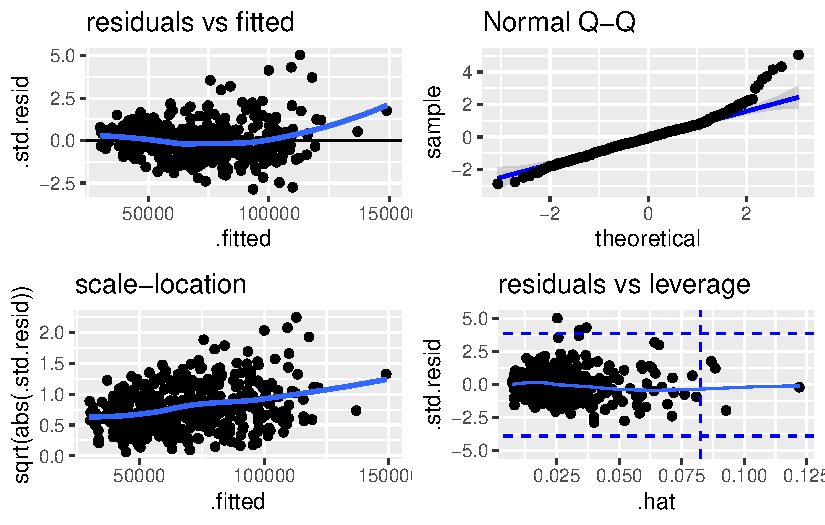
\includegraphics[keepaspectratio]{main_files/figure-pdf/unnamed-chunk-9-1.pdf}}

A partir da análise dos gráficos de resíduos, percebemos que o modelo
proposto não estava adequado, e resolvemos partir para a abordagem
seguinte:

\pandocbounded{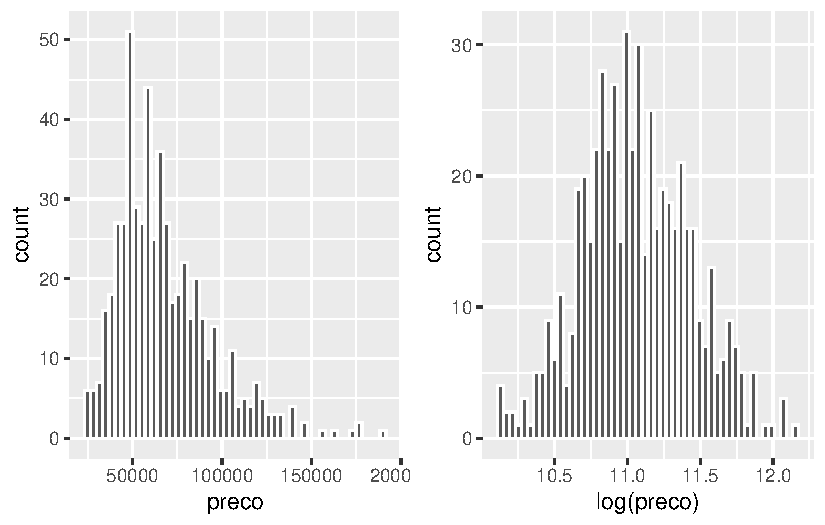
\includegraphics[keepaspectratio]{main_files/figure-pdf/unnamed-chunk-10-1.pdf}}

\begin{Shaded}
\begin{Highlighting}[]
\NormalTok{log\_wflow }\OtherTok{\textless{}{-}} \FunctionTok{workflow}\NormalTok{() }\SpecialCharTok{|\textgreater{}}
  \FunctionTok{add\_model}\NormalTok{(lm\_model) }\SpecialCharTok{|\textgreater{}}
  \FunctionTok{add\_formula}\NormalTok{(}\FunctionTok{log}\NormalTok{(preco) }\SpecialCharTok{\textasciitilde{}}\NormalTok{ .)}
\NormalTok{lmlog\_fit }\OtherTok{\textless{}{-}} \FunctionTok{fit}\NormalTok{(log\_wflow, }\AttributeTok{data =}\NormalTok{ treino)}
\NormalTok{fit2 }\OtherTok{\textless{}{-}} \FunctionTok{extract\_fit\_engine}\NormalTok{(lmlog\_fit)}
\FunctionTok{anova}\NormalTok{(fit2)}
\end{Highlighting}
\end{Shaded}

\begin{verbatim}
Analysis of Variance Table

Response: ..y
                      Df  Sum Sq Mean Sq  F value    Pr(>F)    
area_lote              1 19.8856 19.8856 434.0958 < 2.2e-16 ***
quartos                1  4.5340  4.5340  98.9751 < 2.2e-16 ***
banheiros              1  4.8898  4.8898 106.7430 < 2.2e-16 ***
andares                1  2.7801  2.7801  60.6880 5.199e-14 ***
entrada_carrosim       1  1.6797  1.6797  36.6671 3.090e-09 ***
area_recreacaosim      1  1.7013  1.7013  37.1384 2.474e-09 ***
poraosim               1  1.4984  1.4984  32.7096 2.023e-08 ***
aquecimento_gassim     1  0.2998  0.2998   6.5447 0.0108663 *  
ar_condicionadosim     1  2.3946  2.3946  52.2727 2.270e-12 ***
vagas_garagem          1  0.8890  0.8890  19.4063 1.340e-05 ***
area_preferencialsim   1  0.6302  0.6302  13.7568 0.0002357 ***
Residuals            424 19.4231  0.0458                       
---
Signif. codes:  0 '***' 0.001 '**' 0.01 '*' 0.05 '.' 0.1 ' ' 1
\end{verbatim}

\begin{Shaded}
\begin{Highlighting}[]
\FunctionTok{ggresiduals}\NormalTok{(fit2)}
\end{Highlighting}
\end{Shaded}

\pandocbounded{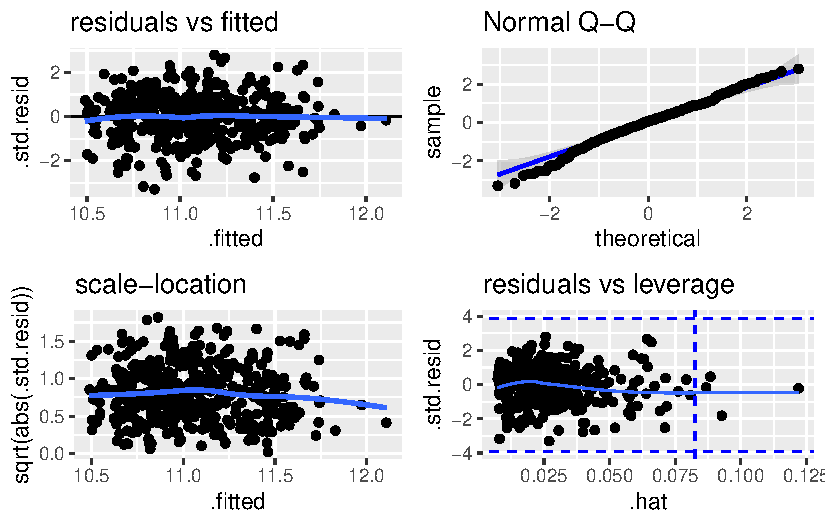
\includegraphics[keepaspectratio]{main_files/figure-pdf/unnamed-chunk-11-1.pdf}}

A alteração realizada no modelo indicou uma melhora ao analisar os novos
gráficos do resíduo, porém ainda incompleto.

\begin{Shaded}
\begin{Highlighting}[]
\NormalTok{fit\_full }\OtherTok{\textless{}{-}} \FunctionTok{lm}\NormalTok{(}\FunctionTok{log}\NormalTok{(preco) }\SpecialCharTok{\textasciitilde{}}\NormalTok{ .}\SpecialCharTok{\^{}}\DecValTok{2}\NormalTok{, }\AttributeTok{data =}\NormalTok{ treino)}

\NormalTok{fit\_SQ }\OtherTok{\textless{}{-}} \FunctionTok{lm}\NormalTok{(}\FunctionTok{log}\NormalTok{(preco) }\SpecialCharTok{\textasciitilde{}}\NormalTok{ . }\SpecialCharTok{+} \FunctionTok{I}\NormalTok{(area\_lote}\SpecialCharTok{\^{}}\DecValTok{2}\NormalTok{),}\AttributeTok{data =}\NormalTok{ treino)}
\FunctionTok{anova}\NormalTok{(fit2, fit\_SQ)}
\end{Highlighting}
\end{Shaded}

\begin{verbatim}
Analysis of Variance Table

Response: ..y
                      Df  Sum Sq Mean Sq  F value    Pr(>F)    
area_lote              1 19.8856 19.8856 434.0958 < 2.2e-16 ***
quartos                1  4.5340  4.5340  98.9751 < 2.2e-16 ***
banheiros              1  4.8898  4.8898 106.7430 < 2.2e-16 ***
andares                1  2.7801  2.7801  60.6880 5.199e-14 ***
entrada_carrosim       1  1.6797  1.6797  36.6671 3.090e-09 ***
area_recreacaosim      1  1.7013  1.7013  37.1384 2.474e-09 ***
poraosim               1  1.4984  1.4984  32.7096 2.023e-08 ***
aquecimento_gassim     1  0.2998  0.2998   6.5447 0.0108663 *  
ar_condicionadosim     1  2.3946  2.3946  52.2727 2.270e-12 ***
vagas_garagem          1  0.8890  0.8890  19.4063 1.340e-05 ***
area_preferencialsim   1  0.6302  0.6302  13.7568 0.0002357 ***
Residuals            424 19.4231  0.0458                       
---
Signif. codes:  0 '***' 0.001 '**' 0.01 '*' 0.05 '.' 0.1 ' ' 1
\end{verbatim}

\begin{Shaded}
\begin{Highlighting}[]
\NormalTok{fit2 }\OtherTok{\textless{}{-}} \FunctionTok{lm}\NormalTok{(}\FunctionTok{log}\NormalTok{(preco) }\SpecialCharTok{\textasciitilde{}}\NormalTok{ ., }\AttributeTok{data =}\NormalTok{ treino)}

\NormalTok{fit\_step }\OtherTok{\textless{}{-}}\NormalTok{ stats}\SpecialCharTok{::}\FunctionTok{step}\NormalTok{(}
\NormalTok{  fit2,}
  \AttributeTok{direction =} \StringTok{"both"}\NormalTok{,}
  \AttributeTok{scope =} \FunctionTok{list}\NormalTok{(}\AttributeTok{upper =} \FunctionTok{formula}\NormalTok{(fit\_full)),}
  \AttributeTok{trace =} \DecValTok{0}
\NormalTok{)}

\NormalTok{lm\_model }\OtherTok{\textless{}{-}} \FunctionTok{linear\_reg}\NormalTok{() }\SpecialCharTok{|\textgreater{}}
  \FunctionTok{set\_engine}\NormalTok{(}\StringTok{"lm"}\NormalTok{)}

\NormalTok{log\_wflow }\OtherTok{\textless{}{-}} \FunctionTok{workflow}\NormalTok{() }\SpecialCharTok{|\textgreater{}}
  \FunctionTok{add\_model}\NormalTok{(lm\_model) }\SpecialCharTok{|\textgreater{}}
  \FunctionTok{add\_formula}\NormalTok{(}\FunctionTok{log}\NormalTok{(preco) }\SpecialCharTok{\textasciitilde{}}\NormalTok{ .)}

\NormalTok{step\_wflow }\OtherTok{\textless{}{-}} \FunctionTok{workflow}\NormalTok{() }\SpecialCharTok{|\textgreater{}}
  \FunctionTok{add\_model}\NormalTok{(lm\_model) }\SpecialCharTok{|\textgreater{}}
  \FunctionTok{add\_formula}\NormalTok{(}\FunctionTok{formula}\NormalTok{(fit\_step))}

\NormalTok{ar\_gr\_wflow }\OtherTok{\textless{}{-}} \FunctionTok{workflow}\NormalTok{() }\SpecialCharTok{|\textgreater{}}
  \FunctionTok{add\_model}\NormalTok{(lm\_model) }\SpecialCharTok{|\textgreater{}}
  \FunctionTok{add\_formula}\NormalTok{(}\FunctionTok{log}\NormalTok{(preco) }\SpecialCharTok{\textasciitilde{}}\NormalTok{ . }\SpecialCharTok{+}\NormalTok{ entrada\_carro}\SpecialCharTok{:}\NormalTok{area\_preferencial)}

\NormalTok{sq\_wflow }\OtherTok{\textless{}{-}} \FunctionTok{workflow}\NormalTok{() }\SpecialCharTok{|\textgreater{}}
  \FunctionTok{add\_model}\NormalTok{(lm\_model) }\SpecialCharTok{|\textgreater{}}
  \FunctionTok{add\_formula}\NormalTok{(}\FunctionTok{log}\NormalTok{(preco) }\SpecialCharTok{\textasciitilde{}}\NormalTok{ . }\SpecialCharTok{+} \FunctionTok{I}\NormalTok{(area\_lote}\SpecialCharTok{\^{}}\DecValTok{2}\NormalTok{))}

\NormalTok{log\_log\_wflow }\OtherTok{\textless{}{-}}\FunctionTok{workflow}\NormalTok{() }\SpecialCharTok{|\textgreater{}}
  \FunctionTok{add\_model}\NormalTok{(lm\_model) }\SpecialCharTok{|\textgreater{}}
  \FunctionTok{add\_formula}\NormalTok{(}\FunctionTok{log}\NormalTok{(preco) }\SpecialCharTok{\textasciitilde{}}\NormalTok{ . }\SpecialCharTok{{-}}\NormalTok{ area\_lote }\SpecialCharTok{+} \FunctionTok{log}\NormalTok{(area\_lote))}

\FunctionTok{set.seed}\NormalTok{(}\DecValTok{64}\NormalTok{)}
\NormalTok{folds }\OtherTok{\textless{}{-}} \FunctionTok{vfold\_cv}\NormalTok{(treino, }\AttributeTok{v =} \DecValTok{10}\NormalTok{)}

\NormalTok{cv\_res }\OtherTok{\textless{}{-}} \FunctionTok{bind\_rows}\NormalTok{(}
  \FunctionTok{fit\_resamples}\NormalTok{(log\_wflow,    }\AttributeTok{resamples =}\NormalTok{ folds) }\SpecialCharTok{|\textgreater{}} \FunctionTok{collect\_metrics}\NormalTok{() }\SpecialCharTok{|\textgreater{}} \FunctionTok{mutate}\NormalTok{(}\AttributeTok{modelo =} \StringTok{"Log linear"}\NormalTok{),}
  \FunctionTok{fit\_resamples}\NormalTok{(step\_wflow,   }\AttributeTok{resamples =}\NormalTok{ folds) }\SpecialCharTok{|\textgreater{}} \FunctionTok{collect\_metrics}\NormalTok{() }\SpecialCharTok{|\textgreater{}} \FunctionTok{mutate}\NormalTok{(}\AttributeTok{modelo =} \StringTok{"Log stepwise"}\NormalTok{),}
  \FunctionTok{fit\_resamples}\NormalTok{(ar\_gr\_wflow,  }\AttributeTok{resamples =}\NormalTok{ folds) }\SpecialCharTok{|\textgreater{}} \FunctionTok{collect\_metrics}\NormalTok{() }\SpecialCharTok{|\textgreater{}} \FunctionTok{mutate}\NormalTok{(}\AttributeTok{modelo =} \StringTok{"Log entrada:area\_pref"}\NormalTok{),}
  \FunctionTok{fit\_resamples}\NormalTok{(sq\_wflow,     }\AttributeTok{resamples =}\NormalTok{ folds) }\SpecialCharTok{|\textgreater{}} \FunctionTok{collect\_metrics}\NormalTok{() }\SpecialCharTok{|\textgreater{}} \FunctionTok{mutate}\NormalTok{(}\AttributeTok{modelo =} \StringTok{"Log Sq\_area"}\NormalTok{),}
  \FunctionTok{fit\_resamples}\NormalTok{(log\_log\_wflow,   }\AttributeTok{resamples =}\NormalTok{ folds) }\SpecialCharTok{|\textgreater{}} \FunctionTok{collect\_metrics}\NormalTok{() }\SpecialCharTok{|\textgreater{}} \FunctionTok{mutate}\NormalTok{(}\AttributeTok{modelo =} \StringTok{"Log log\_area"}\NormalTok{)}
  
\NormalTok{) }\SpecialCharTok{|\textgreater{}}
  \FunctionTok{select}\NormalTok{(modelo, .metric, mean, std\_err) }\SpecialCharTok{|\textgreater{}}
  \FunctionTok{pivot\_wider}\NormalTok{(}\AttributeTok{names\_from =}\NormalTok{ .metric, }\AttributeTok{values\_from =} \FunctionTok{c}\NormalTok{(mean, std\_err)) }\SpecialCharTok{|\textgreater{}}
\NormalTok{  knitr}\SpecialCharTok{::}\FunctionTok{kable}\NormalTok{(}\AttributeTok{digits =} \DecValTok{4}\NormalTok{)}
\NormalTok{cv\_res}
\end{Highlighting}
\end{Shaded}

{\def\LTcaptype{none} % do not increment counter
\begin{longtable}[]{@{}lrrrr@{}}
\toprule\noalign{}
modelo & mean\_rmse & mean\_rsq & std\_err\_rmse & std\_err\_rsq \\
\midrule\noalign{}
\endhead
\bottomrule\noalign{}
\endlastfoot
Log linear & 0.2176 & 0.6616 & 0.0092 & 0.0248 \\
Log stepwise & 0.2159 & 0.6626 & 0.0096 & 0.0277 \\
Log entrada:area\_pref & 0.2176 & 0.6615 & 0.0091 & 0.0246 \\
Log Sq\_area & 0.2154 & 0.6675 & 0.0091 & 0.0264 \\
Log log\_area & 0.2142 & 0.6700 & 0.0091 & 0.0270 \\
\end{longtable}
}

\begin{Shaded}
\begin{Highlighting}[]
\CommentTok{\# Ajuste pelo tidymodels}
\NormalTok{res\_log  }\OtherTok{\textless{}{-}} \FunctionTok{last\_fit}\NormalTok{(log\_wflow, }\AttributeTok{split =}\NormalTok{ divisao)}
\NormalTok{res\_step }\OtherTok{\textless{}{-}} \FunctionTok{last\_fit}\NormalTok{(step\_wflow, }\AttributeTok{split =}\NormalTok{ divisao)}
\NormalTok{res\_ar\_gr }\OtherTok{\textless{}{-}} \FunctionTok{last\_fit}\NormalTok{(ar\_gr\_wflow, }\AttributeTok{split =}\NormalTok{ divisao)}
\NormalTok{res\_SQ }\OtherTok{\textless{}{-}} \FunctionTok{last\_fit}\NormalTok{(sq\_wflow, }\AttributeTok{split =}\NormalTok{ divisao)}
\NormalTok{res\_log\_log }\OtherTok{\textless{}{-}} \FunctionTok{last\_fit}\NormalTok{(log\_log\_wflow, }\AttributeTok{split =}\NormalTok{ divisao)}

\CommentTok{\# Tabela para comparação}
\FunctionTok{bind\_rows}\NormalTok{(}
  \FunctionTok{collect\_metrics}\NormalTok{(res\_log)  }\SpecialCharTok{|\textgreater{}} \FunctionTok{mutate}\NormalTok{(}\AttributeTok{modelo =} \StringTok{"Log Linear"}\NormalTok{),}
  \FunctionTok{collect\_metrics}\NormalTok{(res\_step) }\SpecialCharTok{|\textgreater{}} \FunctionTok{mutate}\NormalTok{(}\AttributeTok{modelo =} \StringTok{"Log Stepwise"}\NormalTok{),}
  \FunctionTok{collect\_metrics}\NormalTok{(res\_ar\_gr) }\SpecialCharTok{|\textgreater{}} \FunctionTok{mutate}\NormalTok{(}\AttributeTok{modelo =} \StringTok{"Log entrada:area\_pref"}\NormalTok{),}
  \FunctionTok{collect\_metrics}\NormalTok{(res\_SQ) }\SpecialCharTok{|\textgreater{}} \FunctionTok{mutate}\NormalTok{(}\AttributeTok{modelo =} \StringTok{"Log SQ\_area"}\NormalTok{),}
  \FunctionTok{collect\_metrics}\NormalTok{(res\_log\_log) }\SpecialCharTok{|\textgreater{}} \FunctionTok{mutate}\NormalTok{(}\AttributeTok{modelo =} \StringTok{"Log Log\_area"}\NormalTok{)}
\NormalTok{) }\SpecialCharTok{|\textgreater{}}
  \FunctionTok{select}\NormalTok{(modelo, .metric, .estimate) }\SpecialCharTok{|\textgreater{}}
  \FunctionTok{pivot\_wider}\NormalTok{(}\AttributeTok{names\_from =}\NormalTok{ .metric, }\AttributeTok{values\_from =}\NormalTok{ .estimate) }\SpecialCharTok{|\textgreater{}}
\NormalTok{  knitr}\SpecialCharTok{::}\FunctionTok{kable}\NormalTok{(}\AttributeTok{digits =} \DecValTok{4}\NormalTok{)}
\end{Highlighting}
\end{Shaded}

{\def\LTcaptype{none} % do not increment counter
\begin{longtable}[]{@{}lrr@{}}
\toprule\noalign{}
modelo & rmse & rsq \\
\midrule\noalign{}
\endhead
\bottomrule\noalign{}
\endlastfoot
Log Linear & 0.2188 & 0.6495 \\
Log Stepwise & 0.2386 & 0.5894 \\
Log entrada:area\_pref & 0.2216 & 0.6414 \\
Log SQ\_area & 0.2173 & 0.6498 \\
Log Log\_area & 0.2127 & 0.6652 \\
\end{longtable}
}

Após a tentativa de aplicar o stepwise encontramos um modelo que,
comparado com o modelo básico
\(R^2_1 = 0{,}5893585 \leq R^2_2 =  0,6495407\), foi descartado.




\end{document}
